\subsection{Funktionen und Oberflächen}
    \label{section:solutionDetailsWebAppFunctions}
    Die Webanwendung soll Nutzern eine größere und zugleich detailliertere
    Übersicht über klassifizierte Seiten verschaffen,
    als dies mit Web Annotationen möglich ist.
    Ihre Informationen bezieht sie dafür von der
    Classification Storage API\footnote{vgl. Kapitel \ref{section:solutionDetailsStorageAPI}}.

    Die erste Oberfläche der Webanwendung ist ein Dashboard
    und ist in Abbildung \ref{image:webAppDashboard} zu sehen.

    \begin{figure}[htb]
        \centering
        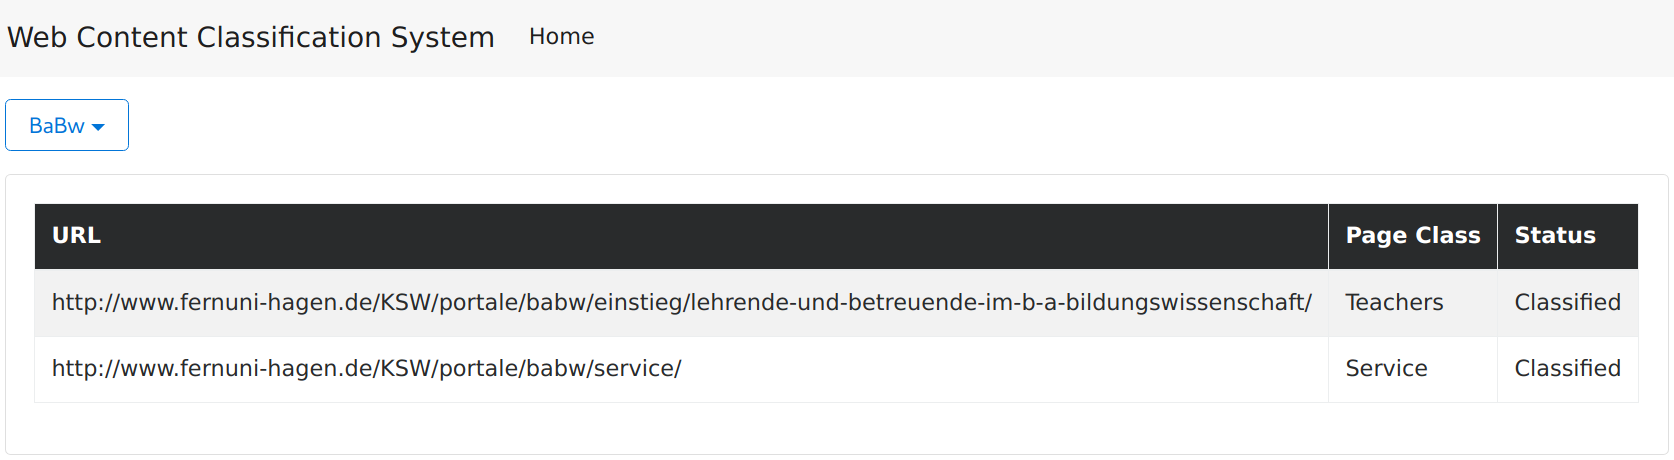
\includegraphics[width=\textwidth]{../resources/web-app/dashboard.png}
        \caption{Dashboard aller klassifizierten Seiten}
        \label{image:webAppDashboard}
    \end{figure}

    Diese Übersichtseite enthält eine Auswahlliste die alle bekannten Sites enthält.
    Bei Auswahl einer Seite, wird die darunter liegende Tabelle mit den Informationen
    der Seiten dieser Site befüllt.
    Besagte Tabelle enthält zu jeder Seite ihre \gls{url}, ihre Klasse und ihren Status.
    Durch einen Klick auf die Zeile einer Seite,
    gelangt man zur Detailseite einer klassifizierten Seite,
    die in Abbildung \ref{image:webAppDetailPage} zu sehen ist.

    \begin{figure}[htb]
        \centering
        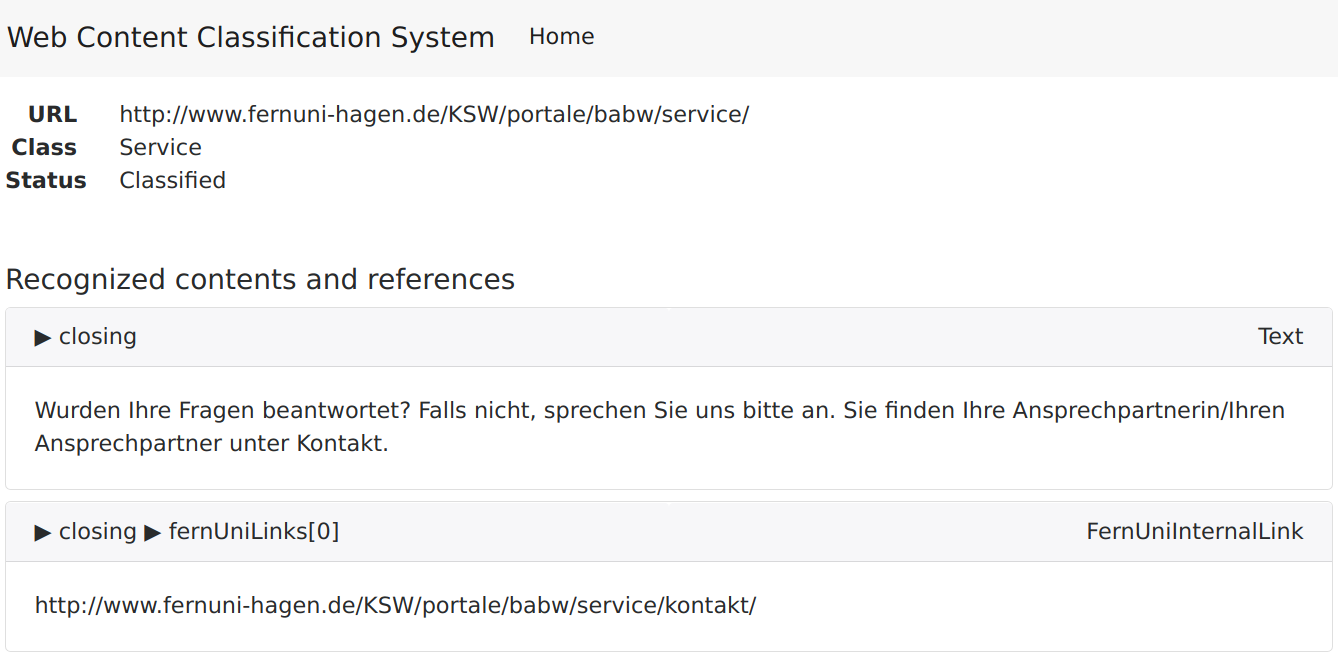
\includegraphics[width=0.8\textwidth]{../resources/web-app/detail-page.png}
        \caption{Detailseite einer klassifizierten Seite}
        \label{image:webAppDetailPage}
    \end{figure}

    Im Kopf dieser Oberfläche sind nochmals die Informationen
    des Dashboards über die aktuelle Klassifikation aufgeführt.
    Darunter befindet sich für jedes Feature ein Abschnitt,
    der verschiedene Informationen zum jeweiligen Feature enthält.
    Oben links ist dies zunächst der Pfad,
    der innerhalb der Klassifikation zu diesem Feature führt.
    Ob es sich um ein Collection Feature handelt,
    kann implizit aus diesem Pfad abgelesen werden,
    da er in diesem Fall den Index des Elementes enthält.
    In Abbildung \ref{image:webAppDetailPage} ist dies am zweiten gelisteten Feature zu sehen.
    Die Klasse des Features ist oben rechts zu sehen.
    Darunter befindet sich der textuelle Inhalt oder das Referenzziel
    des Features.
    Diese Oberfläche verzichtet bewusst darauf auch die Selektoren der Features aufzuführen,
    da diese Informationen für die manuelle Prüfung der Klassifikation weniger wichtig ist
    als die korrekte Einteilung und Strukturierung der Inhalte und Referenzen in Klassen.
